% !TEX encoding = UTF-8
% Title and Authors
\newcommand{\mytitle}{Tracker Project }
\ihead[]{\small \mytitle}
\title{\mytitle}

%%%%%%%%%%%Enter your names here%%%%%%%%
\author{\textbf{Juan Loja (lojag95@cse.yorku.ca)}
\and \textbf{Sadman Sakib Hasan (cse23152@cse.yorku.ca)}
}
%%%%%%%%%%%%%%%%%%%%%%%%%%%%%%%
\date{\today} % Display a given date or no date
\maketitle

\subsection*{Statistics.}
\begin{itemize}
\itemsep0em 
  \item Under which account submitted Prism: cse23152
  \item Under which account submitted Moodle: Hasan, Sadman Sakib
  \item Implementation Language: Eiffel
  \item Estimate hours on requirements document: 20 hours
  \item Estimate of hours on coding and acceptance testing: 32 hours
  \item Hours on debugging and testing: 20 hours out of 32 hours
  \item What was the hardest part of the project?: Developing the the TLA+ specefication
\end{itemize}


\subsection*{Revisions.}

%%%%%%%%%%%%Table of revisions%%%%%%%%
\begin{tabular}{|l|l|p{3in}|}
\hline
Date & Revision & Description \\ 
\hline
14 November  2017
& 1.0
& Add initial Use Case Diagram and Textual Description\\ 
\hline
15 November  2017
& 1.1
& Add Abstract Grammar, Acceptance Test and Safety Invariant\\ 
\hline
28 November  2017
& 2.0
& Add E/R Descriptions\\ 
\hline
29 November  2017
& 2.1
& Add additional Use Case Textual Descriptions\\ 
\hline
2 December  2017
& 3.0
& Add complete TLA+ Specification\\ 
\hline
\end{tabular}

%%%%%%%%%%%%%%%%%%%%%%%%%%%%%%%%
\newpage

\vspace*{2in}
\begin{center}
\huge{\textbf{Requirements Document}:\\ Tracker System}
\end{center}

\newpage
%%%%%%%%%%%%%%%%%%%%%%%%%%%%%%%
\newpage
\tableofcontents
\listoffigures
\listoftables
\newpage
%%%%%%%%%%%%%%%%%%%%%%%%%%%%%%%%%

\section{Informal description of nuclear waste tracker}
A tracker system monitors the position of waste products in nuclear plants and ensures their safe handling. Our customer requires a software system that operators use to manage safe tracking of radioactive waste in their various nuclear plants. We have so far elicited the following information from our customer. 

\begin{figure}[hbt]
\begin{center}
  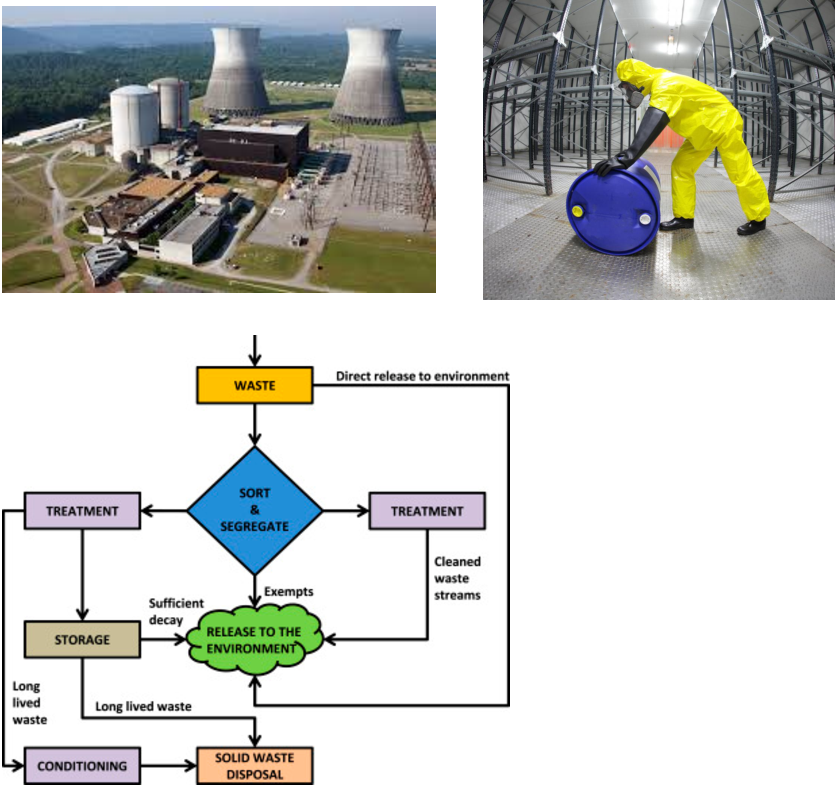
\includegraphics[width=.7\textwidth]{images/waste.pdf}
\end{center}
\end{figure}

Containers of material pass through various stages of processing in the tracking part of the nuclear plant. The tracking plant consist of a number of phases usually corresponding to the physical processes that handle the radioactive materials. Not all plants have precisely the same phases.

As an example, containers (containing a a possibly radioactive material type) might arrive at an initial unpacking phase where they are stored for further processing depending on their material contents. All nuclear plants have only the following types of material: \textit{glass}, \textit{metal}, \textit{plastic}, or \textit{liquid}. No other materials are tracked. 

A subsequent phase might be called the ``assay" phase to measure the recoverable material content of each container before passing onto the next phase. A next stage might be  a compacting phase. A compacting phase might involve dissolving metal contents or crushing glass. Not all material types can necessarily be handled in a phase. For example, we should not move containers with liquid into a compacting phase.  Finally the products of the process might be placed in storage. There may be other phases in a particular instance of the tracker. 

Each container has a unique identifier and contains only one type of material. It is labelled with a preliminary radiation count (in \textit{mSv}). When a container is registered in the system, it is also placed in a phase (not necessarily an initial phase). 

The sievert (symbol: Sv) is a unit of ionizing radiation dose in the International System of Units (SI) and is a measure of the health effect of radiation on the human body. Quantities that are measured in sieverts are intended to represent the stochastic health risk, which for radiation dose assessment is defined as the probability of cancer induction and genetic damage. One sievert carries with it a 5.5\% chance of eventually developing cancer.\footnote{\url{https://en.wikipedia.org/wiki/Sievert}}

For a given plant,  there is an initial setup of two important fixed global parameters for a given plant: there is a limit on the maximum radiation in any phase of the plant (in units of mSv), and there is also a limit on the maximum radiation that any container in the plant may have (in mSv). An error status message shall be signalled if there is an attempt to register a new container in the system with radiation that exceeds the container limit. 

Another operation is to add a new phase (this is information provided by the Domain experts). Requirements elicitation so far yields that a new phase is specified by a phase ID, a name (e.g. "compacting"), a limit on the maximum number of containers in the phase, and a list of material types that may be treated in the phase. A phase may also be removed if there are no containers anywhere in the system. Also, it is possible for an operator to move a container from one phase to another. 

Obviously when dealing with dangerous materials is very important to ensure that no material goes missing and that care is taken to avoid too much material getting into a phase, in case there is a buildup of dangerous substances in one area. The tracking manager is responsible for giving permission to movements of containers between processing phases in order to avoid dangerous situations.

%%%%%%%%%%%%%%%%%%%%%%%%%%%%%%%%%%%%%%%%%%%%%%%%%%%%%%%%%%%%%%%%%%%%%%%%%
\newpage
\section{High level goals}
The high level goals for the System Under Description are:

\begin{description}
  \item[G1:] The operator should be able to safely manage tracking of radioactive waste in their nuclear plants.
  \item[G2:] The cost of manufacturing the tracking system should be as low as possible.
\end{description}

 
%%%%%%%%%%%%%%%%%%%%%%%%%%%%%%%%%%%%%%%%%%%%%%%%%%%%%%%%%%%%%%%%%%%%%%%%%
\newpage
\section{Use Case Diagram and Textual Use Cases}

The next two pages include the use case textual representation of a particular use case \ref{tbl:uc1td} and the use case diagram \ref{fig:uc_diagram} for the System Under Description.\\

\smallskip
\noindent An additional use case (UC-2) is included in the appendix \ref{add-uctd}. The normal flow of the use case in \ref{tbl:uc1td} \textit{includes} calling UC-2.

\begin{table}[h]
\begin{center}
\begin{tabular}{|l|l|}
\hline
\textbf{Use Case ID:} UC-1 \\ \hline
\textbf{Use Case Name:} Move a container \\ \hline
\textbf {Primary Actor:} Operator \\ \hline
\textbf {Secondary Actor:} Tracking Manager \\ \hline
\textbf{Description:} The Operator specifies the option to move a container from a \\desired phase to a destination phase by entering the container id and the \\source and destination phase IDs. The system processes the input and asks \\the Tracking Manager to verify the movement. \\ \hline
\textbf{Scenario:} Sunny Day \\ \hline
\textbf{Trigger:} Operator indicates to move a container.\\ \hline
\textbf{Priority:} High \\ \hline
\textbf{Precondition:}
\\ PRE-1. Container \emph{c} exists in the tracker.
\\ PRE-2. Container \emph{c} is in phase \emph{p1}.
\\ PRE-3. Container \emph{c} is not in phase \emph{p2}.
\\ PRE-4. The material type of \emph{c} is in the list of acceptable materials of \emph{p2}. \\ \hline
\textbf{Postcondition:}
\\ POST-1. Container \emph{c} is in phase \emph{p2}.
\\ POST-2. Container \emph{c} is not in phase \emph{p1}. \\ \hline
\textbf{Normal Flow: 1.0 Move a container, \emph{c}, from phase \emph{p1} to a phase \emph{p2}}
\\ 1. Operator selects the option to move a container from the current phase to \\a new phase.
\\ 2. The System prompts the Operator to enter the ID of the container to be \\moved, the phase ID of the source and destination phase.
\\ 3. Operator enters the ID of the container to be moved and the source and \\destination phase IDs.
\\ 4. System processes the input, finds the destination phase and confirms the \\number of containers in the destination phase has not reached its limit.
\\ 5. System sends a request to the Tracking Manager for the verification of the \\container movement.
\\ 6. System triggers use case UC-2. (Inclusion Point)
\\ 7. System responses OK and provides the status of the container to the Operator \\and Tracking Manager.  \\ \hline
\textbf{Exception Flow: 1.0.E1 Destination phase ID is not in the tracker}
\\ 1. System displays error \textbf{e9: phase identifier not in the system}.
\\ 2. System asks the Operator if they want to try another phase (3a) or to \\exit (4a).
\\ 3a. Operator requests to try another destination phase.
\\ 3b. System starts normal flow over.
\\ 4a. Operator asks to exit.
\\ 4b. System terminates the use case.\\ \hline
\end{tabular}
\end{center}
\caption {UC-1 Textual Description}
\label{tbl:uc1td}
\end{table}

\clearpage
\newpage

\begin{figure}[!htb]
\begin{center}
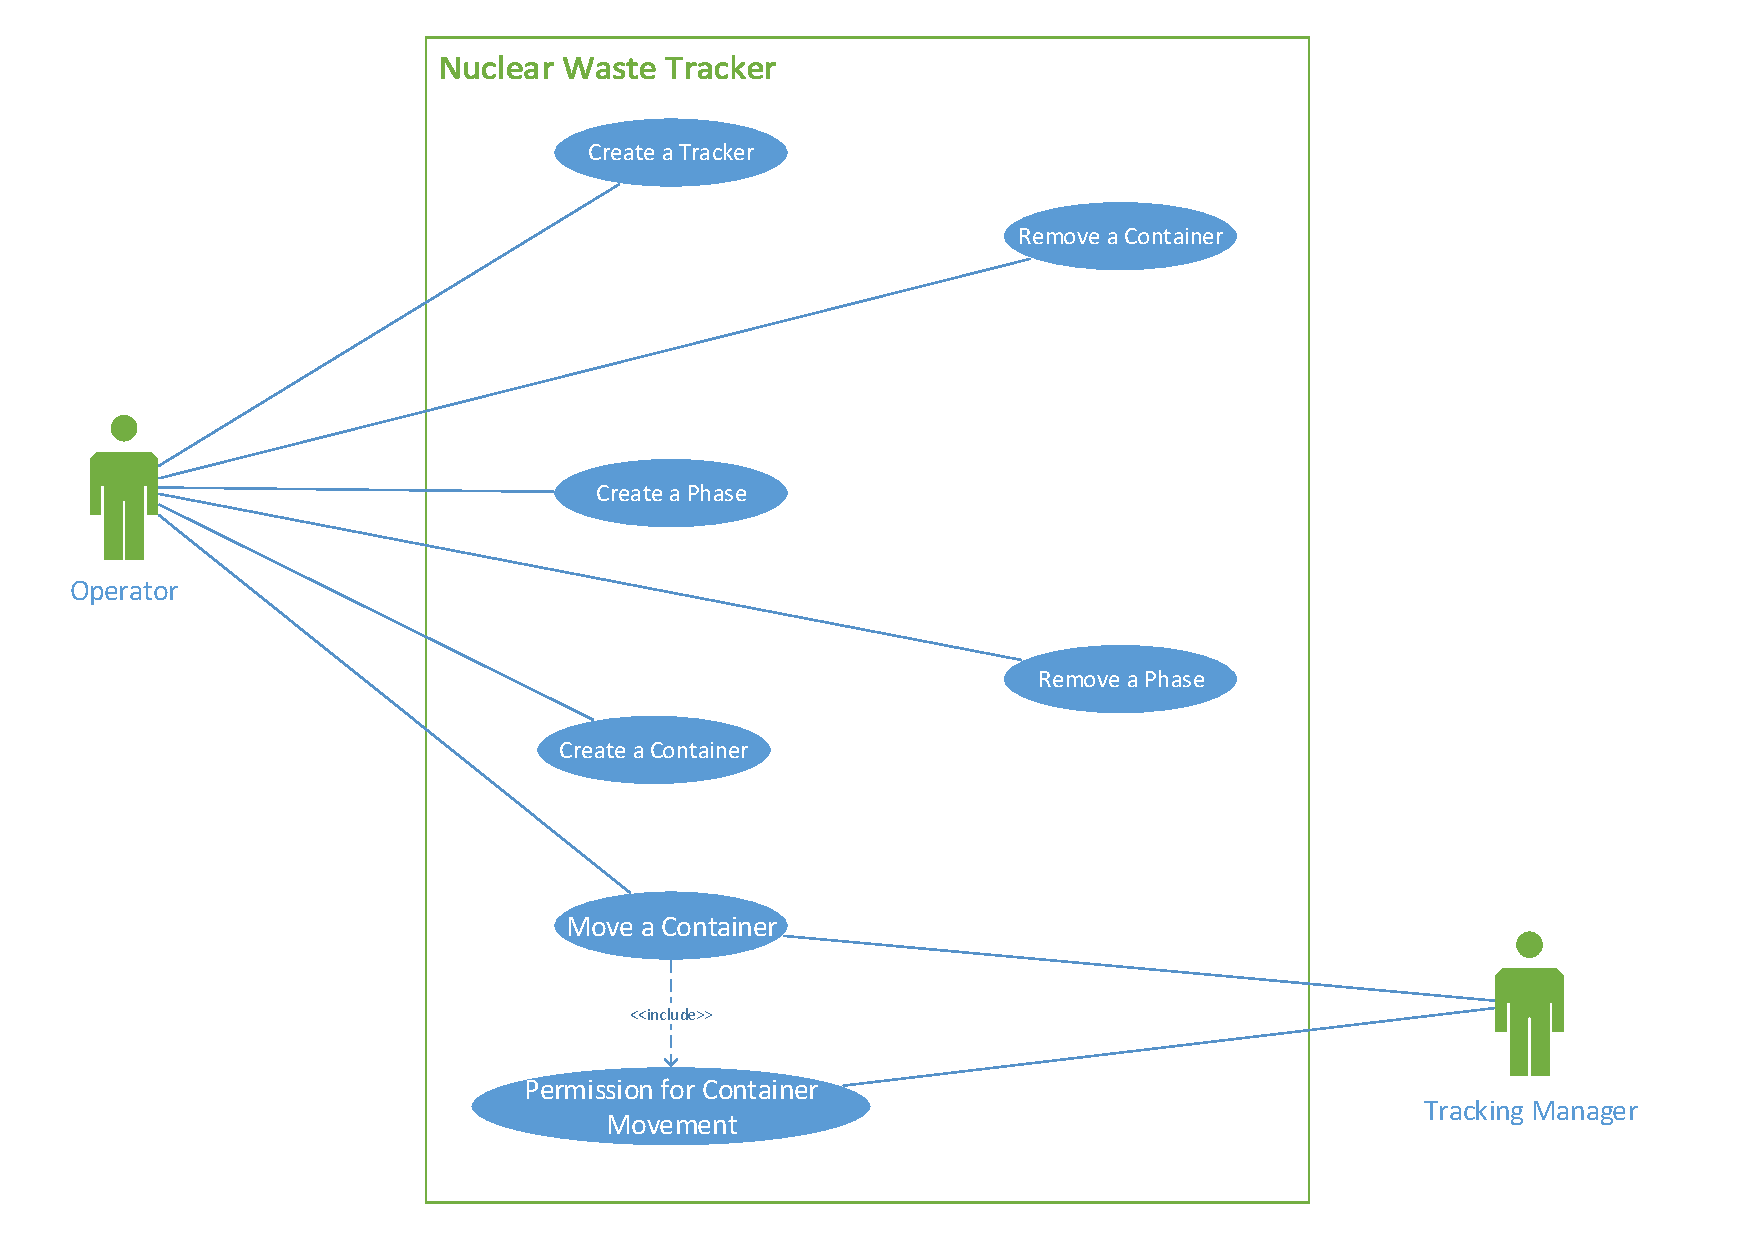
\includegraphics[width=.99\textwidth]{images/uc_diagram.pdf}
\end{center}
\caption{Use Case Diagram}
\label{fig:uc_diagram}
\end{figure}

%%%%%%%%%%%%%%%%%%%%%%%%%%%%%%%%%%%%%%%%%%%%%%%%%%%%%%%%%%%%%%%%%%%%%%%%%
\newpage
\section{E-Descriptions}

Below are \textit{three} E-Descriptions for the System Under Description.

\edescription
{All nuclear plants must only allow the following types of material to be tracked: \textit{glass}, \textit{metal}, \textit{plastic}, or \textit{liquid}.\\}
{}
\label{E1}

\smallskip
\noindent \textbf{Rationale}: The tracking system will only track materials of type: \textit{glass}, \textit{metal}, \textit{plastic}, or \textit{liquid}. Any other materials are not to be tracked.

\edescription
{The tracking manager must be responsible for permitting to move a container from one phase to another.\\}
{}
\label{E2}

\smallskip
\noindent \textbf{Rationale}: When dealing with dangerous materials it is important to ensure that no material goes missing and that care is taken to avoid too much material getting into a phase, in case there is a buildup of dangerous substances in one area.

\edescription
{Materials of a container will be placed in storage once it has passed through various stages of processing.\\}
{}
\label{E2}

\smallskip
\noindent \textbf{Rationale}: The material inside a container might be placed in a storage before sending it out for disposal. This is to be completed once the container has passed through various stages of processing.


%%%%%%%%%%%%%%%%%%%%%%%%%%%%%%%%%%%%%%%%%%%%%%%%%%%%%%%%%%%%%%%%%%%%%%%%%

%%%%%%%%%%%%%%%%%%%%%%%%%%%%%%%%%%%%%%%%%%%%%%%%%%%%%%%%%%%%%%%%%%%%%%%%%
\newpage
\section{R-Descriptions}

Below are \textit{three} R-Descriptions for the System Under Description. Additional R-Descriptions are specified in the appendix \ref{add-rdesc}.


\rdescription
{A given plant shall have two important fixed global parameters: \textit{maximum phase radiation} and \textit{maximum container radiation}.\\}
{}
\label{R1}

\smallskip
\noindent \textbf{Rationale}: Each plant must have a fixed maximum phase and container radiation value fixed. The value should be in units of mSv. The sievert (symbol: Sv) is a unit of ionizing radiation dose in the International System of Units (SI) and is a measure of the health effect of radiation on the human body. Quantities that are measured in sieverts are intended to represent the stochastic health risk, which for radiation dose assessment is defined as the probability of cancer induction and genetic damage.

\rdescription
{Each phase in a plant shall have an unique identifier, a name, limit on the maximum number of containers and list of material types to be treated in that phase.\\}
{}
\label{R2}

\smallskip
\noindent \textbf{Rationale}: Each phase in a plant must be associated with an unique identifier. Along with an unique identifier, it should also have a name, maximum number of containers allowed in the phase and the list of material types that can be treated in the phase.

\rdescription
{A container shall be placed in a phase when registered in a plant.\\}
{}
\label{R3}

\smallskip
\noindent \textbf{Rationale}: When a container is first registered in a plant, it is placed in a phase of the operators wish. The phase does not necessarily have to be the initial phase.


%%%%%%%%%%%%%%%%%%%%%%%%%%%%%%%%%%%%%%%%%%%%%%%%%%%%%%%%%%%%%%%%%%%%%%%%%

\newpage
\section{Abstract UI Grammar for Monitored Events}

After several rounds of requirements elicitation, the following user inputs are defined.

\begin{events}
system tracker -- tracking system for a nuclear plant
type CID = STRING -- container identifiers
type PID = STRING -- phase identifiers
type MATERIAL = {glass, metal, plastic, liquid}
type CONTAINER = TUPLE[material: MATERIAL; radioactivity: VALUE]

new_tracker( -- create a new tracking system
	  max_phase_radiation: VALUE 
	  	-- max radiation allowed for all containers in a phase
	; max_container_radiation: VALUE 
		-- max radation allowed in a container
	)

new_phase( -- create a new phase
	  pid: PID            -- phase identifier
	; phase_name: STRING 
	; capacity: INT       -- number of containers phase handels
	; expected_materials: ARRAY[MATERIAL]  -- subset of materials
)

-- remove a phase with phase identifier pid
remove_phase(pid: PID)

new_container ( -- create a new container and move it to a phase
	  cid: CID  -- container identifier
	; c: CONTAINER
	; pid:PID
	)

remove_container (cid: CID) -- remove a container with container identifier cid

move_container ( -- move a container from source phase to target phase
	  cid: CID   -- container identifier to be moved
	; pid1: PID  -- source phase
	; pid2: PID  -- target phase
	)
\end{events}

%%%%%%%%%%%%%%%%%%%%%%%%%%%%%%%%%%%%%%%%%%%%%%%%%%%%%%%%%%%%%%%%%%%%%%%%
\newpage
\section{Output and Abstract Variables}

Below is the TLA+ analysis of the system. The informal table provides (a) the type of each variable and (b) a description explaining the role of each variable in the abstract state for the tracker, and its initial value in the TLA+ model

\bigskip\bigskip

\begin{table}[h]
\centering
\begin{tabular}{|l|l|l|}
\hline
\rowcolor[HTML]{EFEFEF} 
\textbf{Abstract Variable} & \textbf{Description}                       & \textbf{Initial value} \\ \hline
$e \in ERROR$              &  \begin{tabular}[c]{@{}l@{}}The error message to be \\displayed\end{tabular}          &   "ok"                 \\ \hline
$pid \subseteq PID$        &  \begin{tabular}[c]{@{}l@{}}The set of phase identifiers \\in the tracker\end{tabular}  &  \{\}               \\ \hline
$cid \subseteq CID$        &  \begin{tabular}[c]{@{}l@{}}The set of container identifiers \\in the tracker\end{tabular} &  \{\} \\ \hline
$phases \in [pid -> PHASE]$        &  \begin{tabular}[c]{@{}l@{}}Function from pid to a \\record of phase\end{tabular}  &  $<>$               \\ \hline
$containers \in [cid -> CONTAINER]$        &  \begin{tabular}[c]{@{}l@{}}Function from cid to a \\record of container\end{tabular}  &  $<>$               \\ \hline
$mpr \in Int$        &  \begin{tabular}[c]{@{}l@{}}The maximum phase radiation \\in the tracker\end{tabular} &  $0$               \\ \hline
$mcr \in Int$        &  \begin{tabular}[c]{@{}l@{}}The maximum container \\radiation in the tracker\end{tabular}  &  $0$               \\\hline
\end{tabular}
\caption {Description of TLA+ Output and Abstract Variables}
\label{tbl:out_abs_vars}
\end{table}

%%%%%%%%%%%%%%%%%%%%%%%%%%%%%%%%%%%%%%%%%%%%%%%%%%%%%%%%%%%%%%%%%%%%%%%%
\newpage
\section{ASCII encoded output of the abstract state}

The delivered program shall execute from a CentOS7 console as follows:

\begin{mdframed}
$>$./tracker.exe -b tests/at0.txt 
\end{mdframed}

A sequence of user commands, e.g. at0.txt below, shall conform to the abstract UI grammar.

\begin{code}
-- Acceptance test for Tracker: at0.txt 
-- ASCII comments may occur at the beginning or in the middle of a line.
-- Very Basic Use Case to:
--	set tracker radiation parameters
--	create some phases
--	add some containers
--	move some containers

-- Phases are sorted by pid
-- Containers are sorted by cid
-- Sorting follows normal lexicographic string rules,
-- so that pid11 is before pid4; use pid04 if you want pid4 earlier. 

-- create a new tracker
-- max. radiation in a phase is 50.0
-- max. radiation in a container is 10.0
new_tracker(50.0, 10.0)

-- add 2 phases each having a container handling capacity of 2:
new_phase("pid2", "compacting", 2, <<glass, metal, plastic>>)
new_phase("pid1", "unpacking", 2, <<glass, metal, plastic, liquid>>)

-- type CONTAINER = TUPLE[material: MATERIAL; radioactivity: VALUE]
-- add some containers
new_container("cid4", [metal,   3.0], "pid1")
new_container("cid1", [glass,   5.5], "pid1")
new_container("cid2", [liquid,  0.5], "pid1") -- e11

-- move some containers
move_container ("cid1", "pid1", "pid2")
move_container ("cid4", "pid1", "pid2")	
\end{code}


The output shall display as follows:

\begin{code}
  state 0 ok
  max_phase_radiation: 0.00, max_container_radiation: 0.00
  phases: pid->name:capacity,count,radiation
  containers: cid->pid->material,radioactivity
->new_tracker(50,10)
  state 1 ok
  max_phase_radiation: 50.00, max_container_radiation: 10.00
  phases: pid->name:capacity,count,radiation
  containers: cid->pid->material,radioactivity
->new_phase("pid2","compacting",2,<<glass, metal, plastic>>)
  state 2 ok
  max_phase_radiation: 50.00, max_container_radiation: 10.00
  phases: pid->name:capacity,count,radiation
    pid2->compacting:2,0,0.00,{glass,metal,plastic}
  containers: cid->pid->material,radioactivity
->new_phase("pid1","unpacking",2,<<glass, metal, plastic, liquid>>)
  state 3 ok
  max_phase_radiation: 50.00, max_container_radiation: 10.00
  phases: pid->name:capacity,count,radiation
    pid1->unpacking:2,0,0.00,{glass,metal,plastic,liquid}
    pid2->compacting:2,0,0.00,{glass,metal,plastic}
  containers: cid->pid->material,radioactivity
->new_container("cid4",[metal, 3],"pid1")
  state 4 ok
  max_phase_radiation: 50.00, max_container_radiation: 10.00
  phases: pid->name:capacity,count,radiation
    pid1->unpacking:2,1,3.00,{glass,metal,plastic,liquid}
    pid2->compacting:2,0,0.00,{glass,metal,plastic}
  containers: cid->pid->material,radioactivity
    cid4->pid1->metal,3.00
->new_container("cid1",[glass, 5.5],"pid1")
  state 5 ok
  max_phase_radiation: 50.00, max_container_radiation: 10.00
  phases: pid->name:capacity,count,radiation
    pid1->unpacking:2,2,8.50,{glass,metal,plastic,liquid}
    pid2->compacting:2,0,0.00,{glass,metal,plastic}
  containers: cid->pid->material,radioactivity
    cid1->pid1->glass,5.50
    cid4->pid1->metal,3.00
->new_container("cid2",[liquid, 0.5],"pid1")
  state 6 e11: this container will exceed phase capacity
->move_container("cid1","pid1","pid2")
  state 7 ok
  max_phase_radiation: 50.00, max_container_radiation: 10.00
  phases: pid->name:capacity,count,radiation
    pid1->unpacking:2,1,3.00,{glass,metal,plastic,liquid}
    pid2->compacting:2,1,5.50,{glass,metal,plastic}
  containers: cid->pid->material,radioactivity
    cid1->pid2->glass,5.50
    cid4->pid1->metal,3.00
->move_container("cid4","pid1","pid2")
  state 8 ok
  max_phase_radiation: 50.00, max_container_radiation: 10.00
  phases: pid->name:capacity,count,radiation
    pid1->unpacking:2,0,0.00,{glass,metal,plastic,liquid}
    pid2->compacting:2,2,8.50,{glass,metal,plastic}
  containers: cid->pid->material,radioactivity
    cid1->pid2->glass,5.50
    cid4->pid2->metal,3.00
\end{code}

%%%%%%%%%%%%%%%%%%%%%%%%%%%%%%%%%%%%%%%%%%%%%%%%%%%%%%%%%%%%%%%%%%%%%%%%
\newpage
\section{TLA+ specfication, invariants and validation}

%\hl{Complete this section.} Ensure that TLA+ specifications don't line wrap, or wrap from one page to %another. Make each page of this document readable on its own. Provide appropriate commentary.

\subsection{Abstract State}

The following are the abstract state variables used in the TLA+ Specification. (For the full TLA+ specification, see Appendix \ref{tla-spec}): \\ 

First is defining $MATERIAL$, $ERROR$, $PHASE$, $CONTAINER$, and $VALUE$:

 \begin{itemize}
\item \textbf{MATERIAL}: Set of all possible materials each container can have
\item \textbf{ERROR}: Set of errors for the tracker
\item \textbf{PHASE}: Set of records containing phase capacity, expected materials, current number of containers in phase, and current radioactivity of phase.
\item \textbf{CONTAINER}: Set of records that has container radioactivity, container material, and the id of the phase that the container is in.
\item \textbf{VALUE}: Allows to abstract real numbers to integers. Radioactivity values are represented as integers. 
\end{itemize}

\begin{figure}[!htb]
\begin{center}
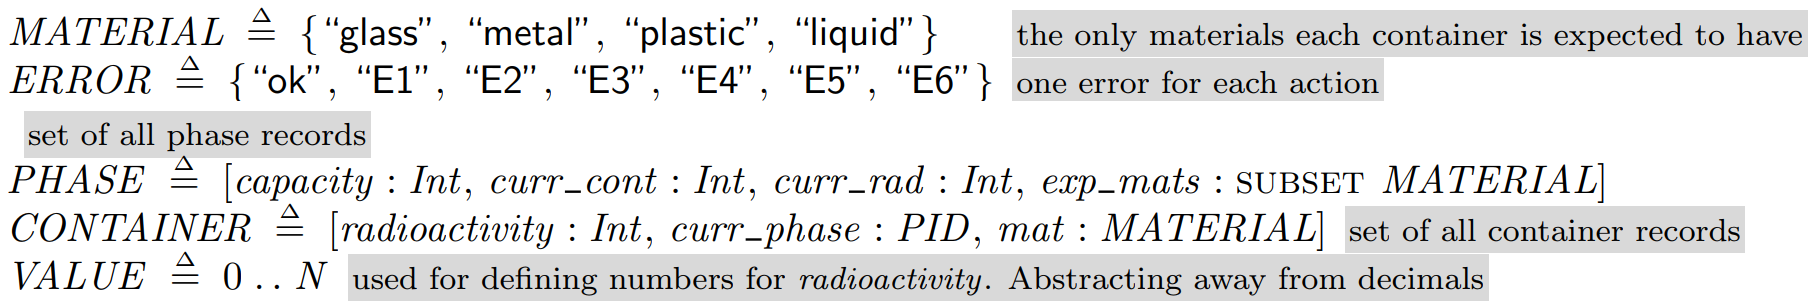
\includegraphics[width=.99\textwidth]{images/tla_defs.png}
\end{center}
\caption{Defining Tracker Types}
\label{fig:defining_tracker}
\end{figure}

\newpage

The following are the variables that define the state of the tracker as well as their type:

\begin{itemize}
\item \textbf{cid}: Set of all container ids in the tracker
\item \textbf{pid}: Set of all phase ids in the tracker
\item \textbf{containers}: Function from cid to a record of container
\item \textbf{phases}: Function from pid to a record of phase
\item \textbf{mpr}: Maximum phase radiation in the tracker
\item \textbf{mcr}: Maximum container radiation in the tracker
\item \textbf{e}: Error message to be displayed
\end{itemize}

\tlatex
\@x{ {\VARIABLES}}%
\@x{\@s{20.5} cid}%
\@x{\@s{16.4} ,\, containers}%
\@x{\@s{16.4} ,\, pid}%
\@x{\@s{16.4} ,\, phases}%
\@x{\@s{16.4} ,\, mpr}%
\@x{\@s{16.4} ,\, mcr}%
\@x{\@s{16.4} ,\, e}%

\@x{ TypeOK \.{\defeq}}%
\@x{\@s{16.4} \.{\land}\@s{9.74} e \.{\in} ERROR}%
\@x{\@s{16.4} \.{\land}\@s{9.74} pid \.{\subseteq} PID}%
\@x{\@s{16.4} \.{\land}\@s{9.74} cid \.{\subseteq} CID}%
\@x{\@s{16.4} \.{\land}\@s{9.74} phases \.{\in} [pid -> PHASE]}%
\@x{\@s{16.4} \.{\land}\@s{9.74} containers \.{\in} [cid -> CONTAINER}%
\@x{\@s{16.4} \.{\land}\@s{9.74} mpr \.{\in} Int}%
\@x{\@s{16.4} \.{\land}\@s{9.74} mcr \.{\in} Int}%



\newpage


\subsection{Abstractions Used}

The main abstraction used in modeling the tracker in TLA+ was using integers instead of real numbers to set the radioactivity value for phases and containers. This was done to make it a bit simple when defining the container, phases, and the tracker itself. Another thing to note is that phase name was not included in the model. This was simply to reduce the amount of elements in the record representing the phase and make the model checker run faster. In addition to this, in the implementation of the tracker, phases and containers were stored in hash maps. In the TLA+ specification, there was a set representing all the current phase ids in the tracker as well as a set of functions with mapping $[pid \to CONTAINER]$. Containers were represented in a similar way. 

\subsection{Safety Invariants}

The following are the safety invariants described in the TLA+ Specification:

\begin{itemize}
\item \textbf{SafeRadioactivity}: Checks if the radioactivity is within the limits of the tracker's maximum radiation level for all phases and containers
\item \textbf{PhasesNotOverCapacity}: Checks if all phases are within their capacity in terms of the maximum containers they can hold
\item \textbf{AllContainersInPhase}: Checks if all containers are in a phase that exists in a tracker
\end{itemize}

\@x{ SafeRadioactivity \.{\defeq}}%
\@x{\@s{16.4} \.{\land}\@s{9.74} \A\, id \.{\in} pid \.{:}
	\.{\land}\@s{9.74} 0 <= phases[id].curr\_rad <= mpr}%
\@x{\@s{16.4} \.{\land}\@s{9.74} \A\, id \.{\in} pid \.{:}
	\.{\land}\@s{9.74} 0 <= containers[id].radioactivity <= mcr} \\

\@x{ PhasesNotOverCapacity \.{\defeq}}%
\@x{\@s{16.4} \A\, id \.{\in} pid \.{:} 0 <= phases[id].curr\_cont <= phases[id].capacity} \\
	
\@x{ AllContainersInPhase \.{\defeq}}%
\@x{\@s{16.4} \A\, id \.{\in} cid \.{:} containers[id].curr\_phasae \.{\in} pid}

\newpage
\subsection{Actions}
The following are the actions for the tracker as specified in TLA: \\

This is the $new\_tracker$ action used to set the maixmum phase and container radioactivity. The gurad checks that the values are non-negative and also makes sure the maximum container radioactivity is not greater than the maximum phase radioactivity. In addition, it checks that there are no containers currently in the tracker. If these conditions are met, the values $mcr$ and $mpr$ are set. The rest of the variables remain unchanged.   

\begin{figure}[!htb]
\begin{center}
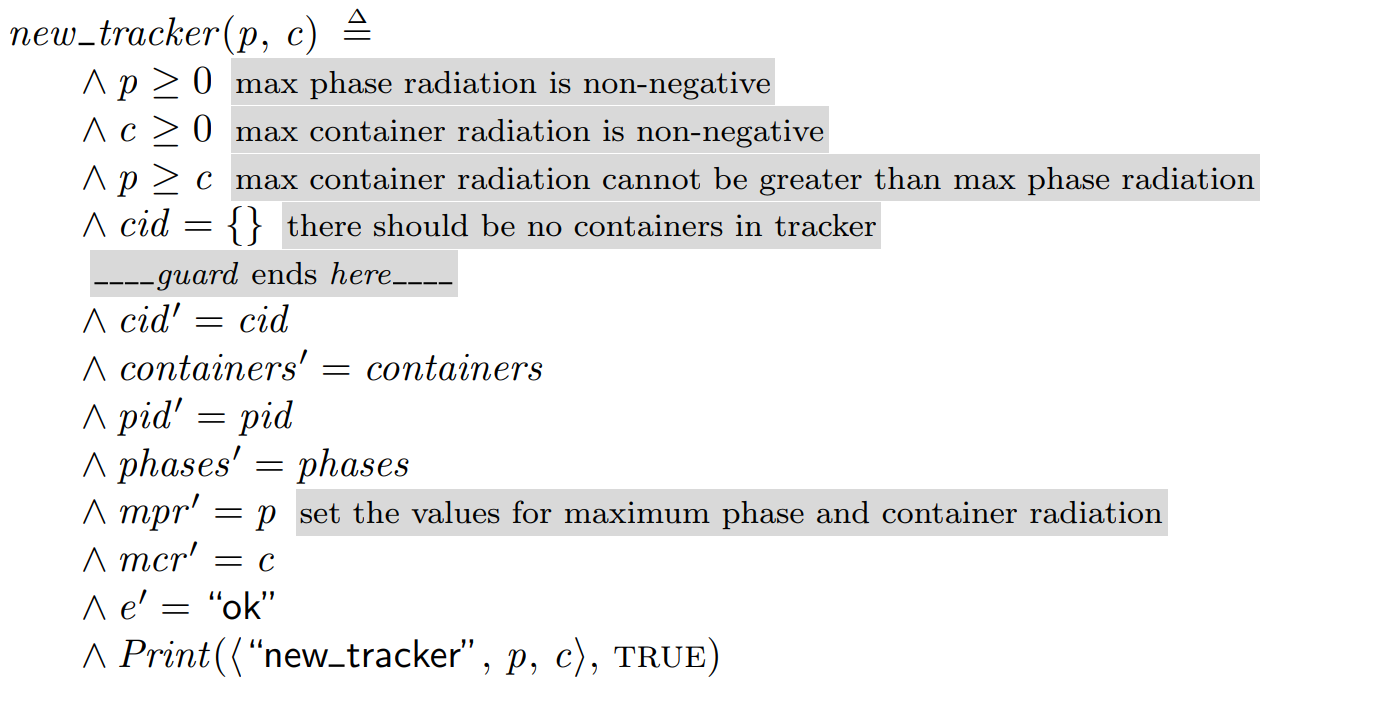
\includegraphics[width=.99\textwidth]{images/new_tracker.png}
\end{center}
\caption{New Tracker Action in TLA}
\label{fig:new_tracker_action}
\end{figure}

\newpage
This is the $new\_phase$ action used to create a new phase in the tracker. The gurad checks that the phase does not exist in the tracker already. It checks that it has a capacity of at least 1. And it also checks that there are no containers currently in the tracker. If these conditions are met, then a new phase id is added to the set of tracker phase ids as well as a new PHASE record. The rest of the variables remain unchanged.   
% This is picture of new _phase action
\begin{figure}[!htb]
\begin{center}
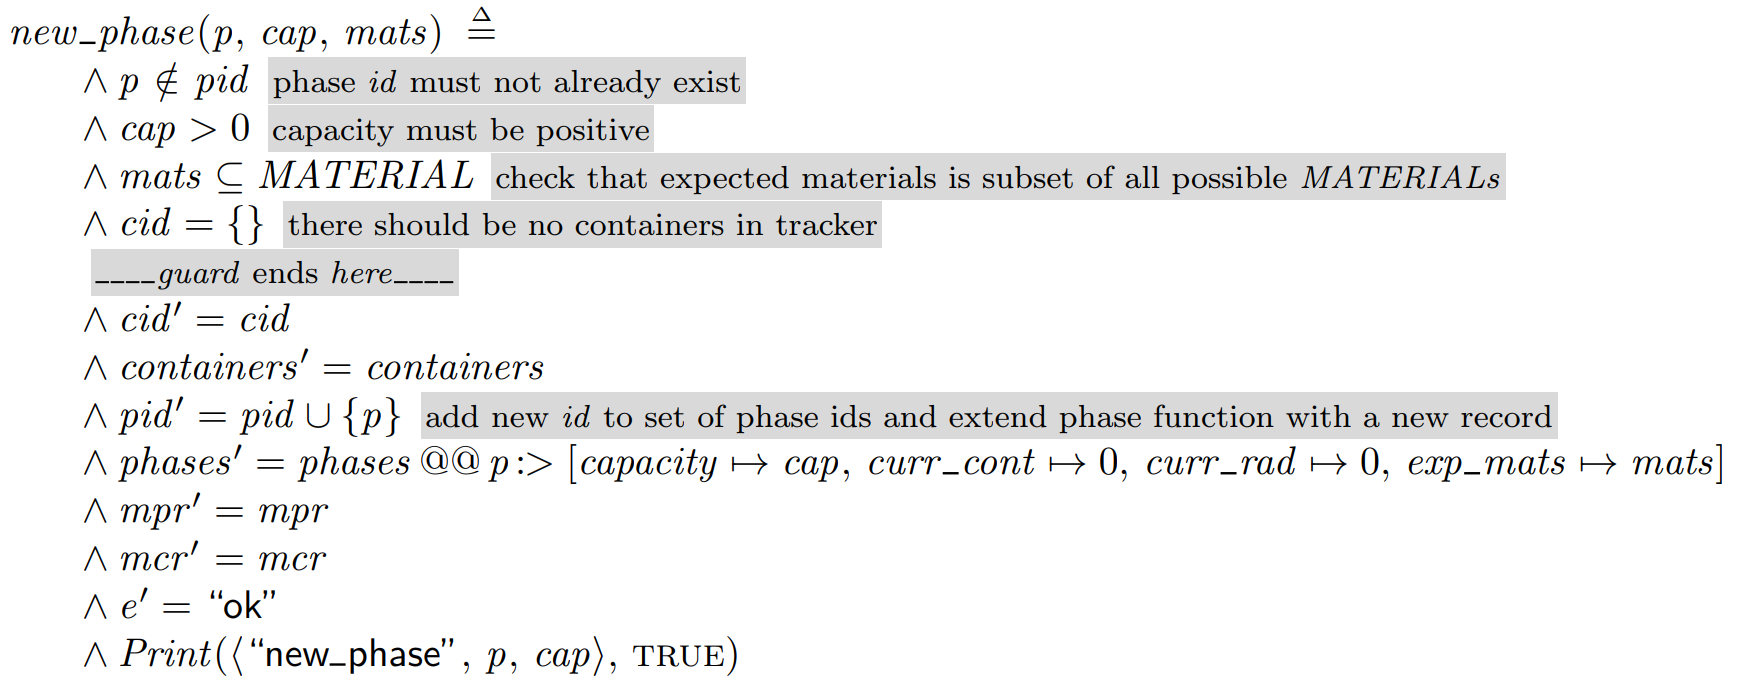
\includegraphics[width=.99\textwidth]{images/new_phase.png}
\end{center}
\caption{New Phase Action in TLA}
\label{fig:new_phase_action}
\end{figure}

\newpage
This is the $new\_container$ action used to create a new container in the tracker. The gurad checks for several things. It checks that this container has not been added before by checking its id. It checks that the destination phase is already in the tracker. It checks that the container doesn't go over radioactivity limit. And finally, it checks if the container can go into the destination phase by checking the capacity, current phase radioactivity, and whether or not the phase accepts the container $MATERIAL$. If these conditions are met, then a new container is added by adding its id to the set of container ids in the tracker. A new $CONTAINER$ record is added and finally, the destination phase is updated accordingly. The rest of the variables remain unchanged.   
% This is picture of new _container action
\begin{figure}[!htb]
\begin{center}
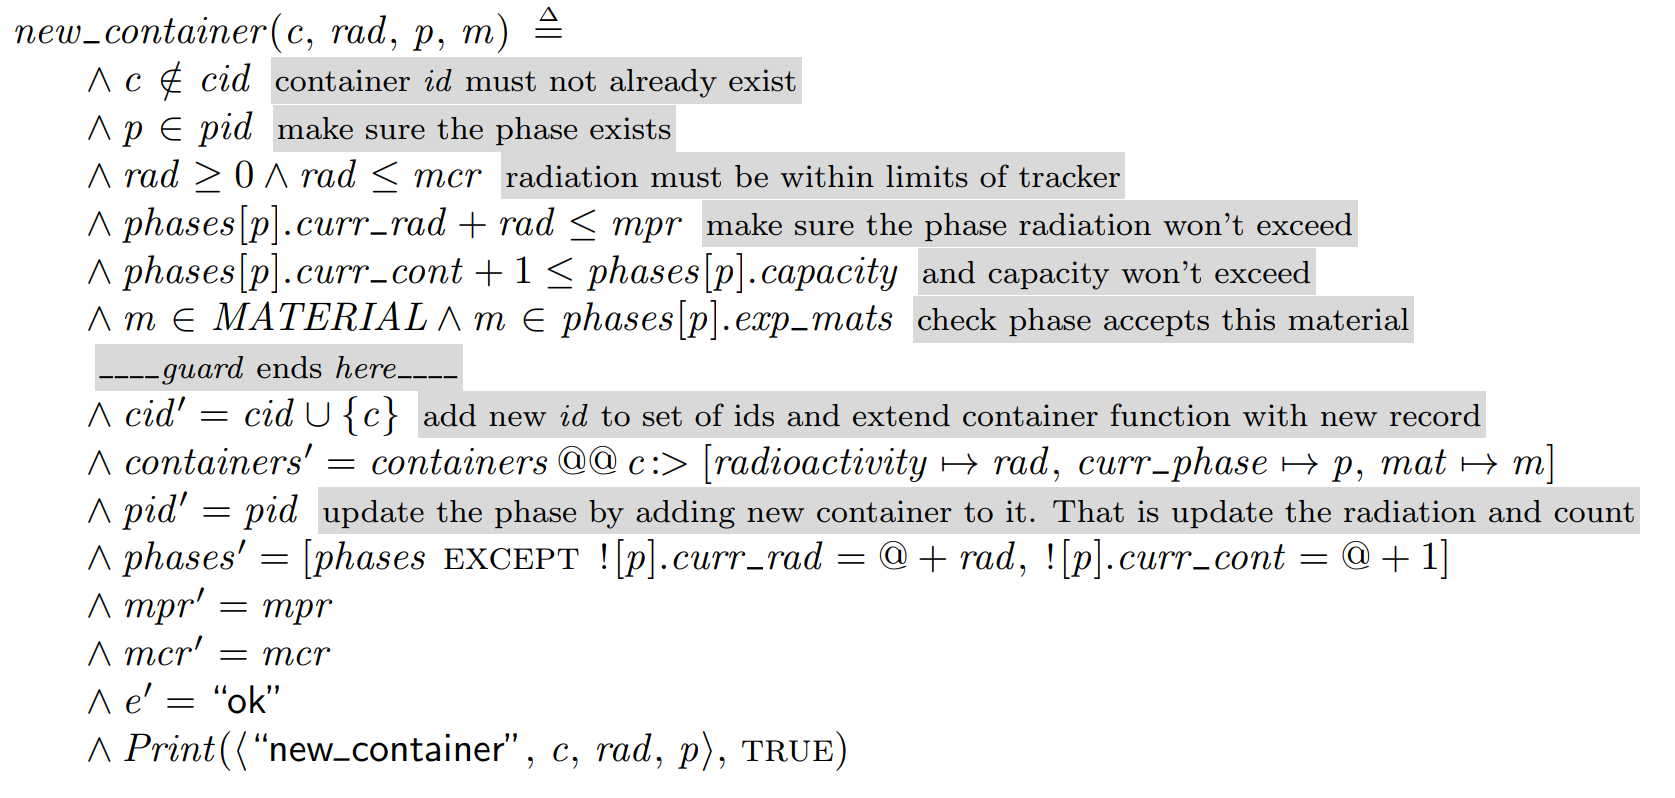
\includegraphics[width=.99\textwidth]{images/new_container.png}
\end{center}
\caption{New Container Action in TLA}
\label{fig:new_container_action}
\end{figure}


\newpage
This is the $remove\_container$ action used to remove an existing container in the tracker. The guard simply checks if the container exists in the tracker. If it does, it removes the container id from the set of container ids in the tracker. It also removes the CONTAINER record. In addition, it updates the phase where the container was currently by removing it from it. The rest of the variables remain unchanged.   
% This is picture of remove_container action
\begin{figure}[!htb]
\begin{center}
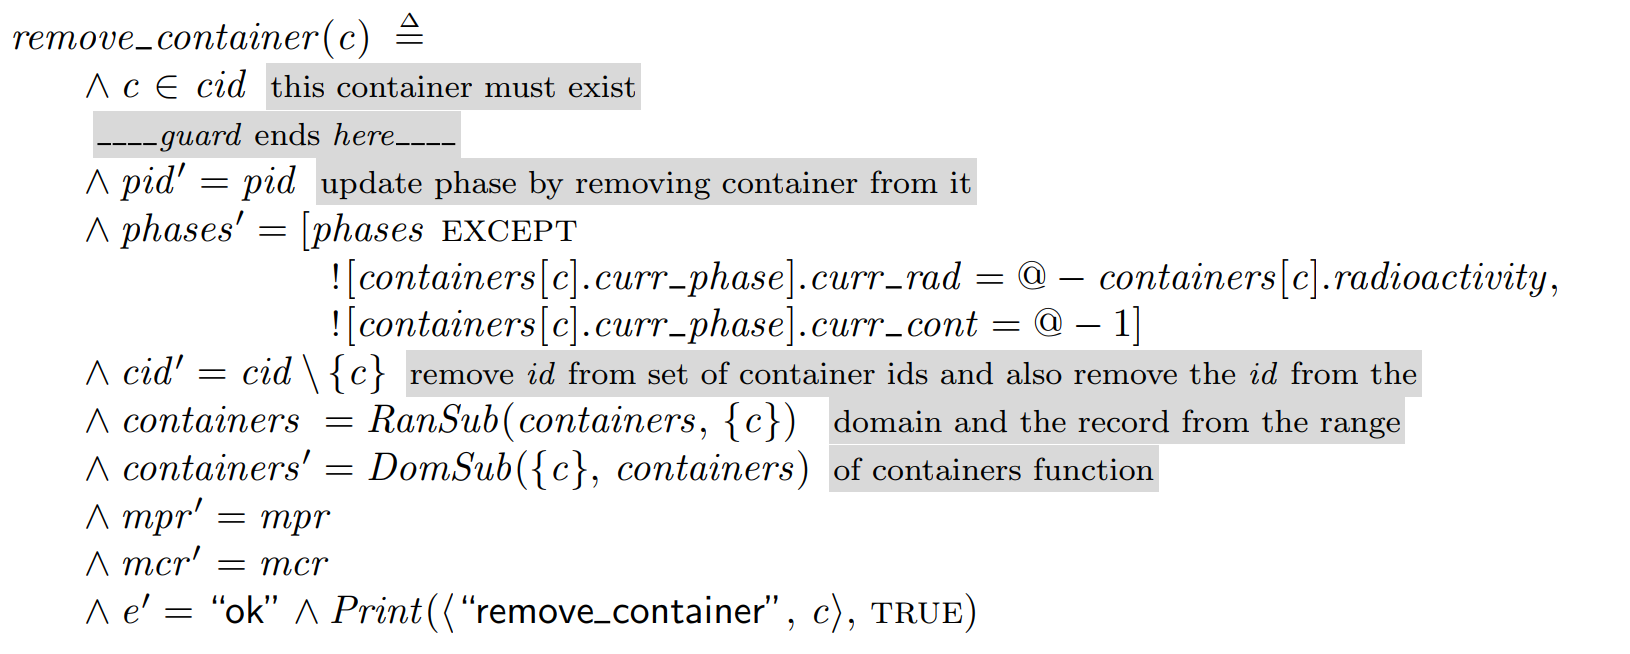
\includegraphics[width=.99\textwidth]{images/remove_container.png}
\end{center}
\caption{Remove Container Action in TLA}
\label{fig:remove_container_action}
\end{figure}

\newpage
This is the $remove\_phase$ action used to remove an existing phase in the tracker. The guard simply checks if the phase exists in the tracker and if there are no containers currently in the tracker. If these conditions are met, the phase id is removed from the set of phase ids in the tracker and the PHASE record is removed as well. The rest of the variables remain unchanged.   
% This is picture of remove_phase action
\begin{figure}[!htb]
\begin{center}
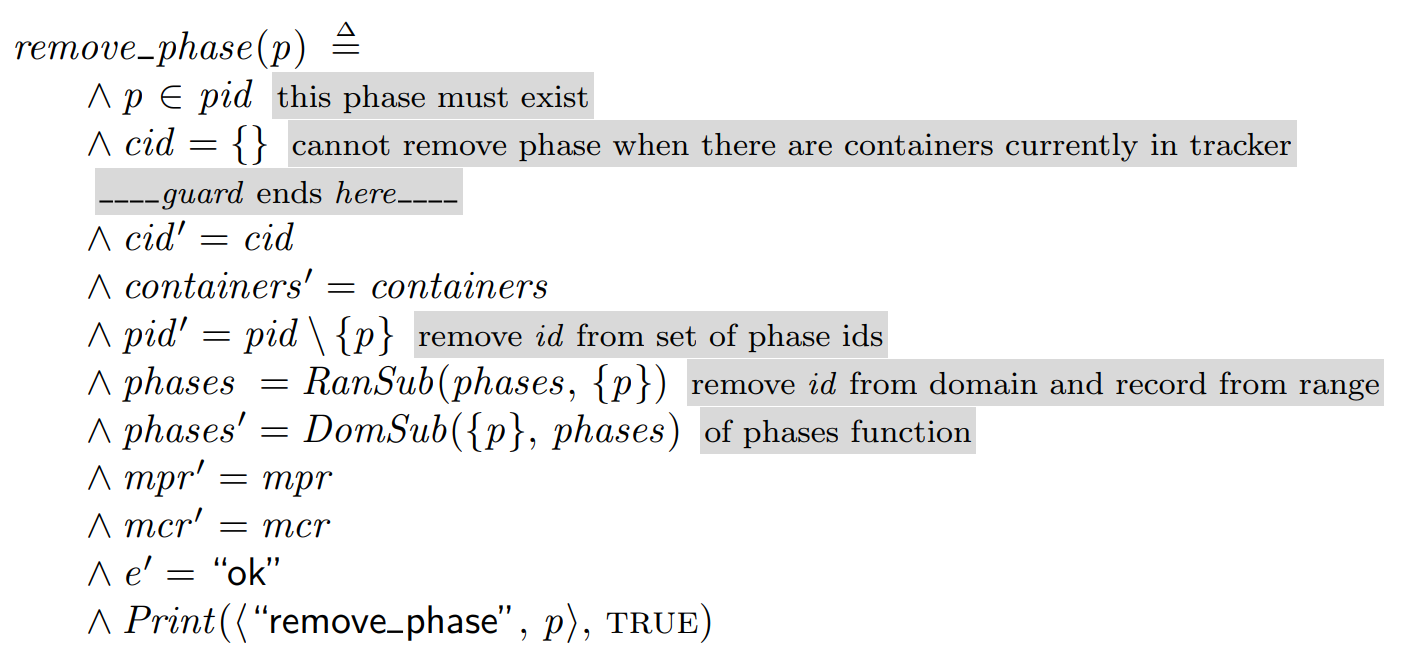
\includegraphics[width=.99\textwidth]{images/remove_phase.png}
\end{center}
\caption{Remove Phase Action in TLA}
\label{fig:remove_phase_action}
\end{figure}

\newpage
This is the $move\_container$ action used to move a container from one phase to another. The guard checks for several things. Firstly it checks if the container, source and target phase exist. Then it checks if the target phase will be able to accept the container. If the conditions are met, the container is removed from the source phase and added to the destination phase. The rest of the variables remain unchanged.   
% This is picture of move action
\begin{figure}[!htb]
\begin{center}
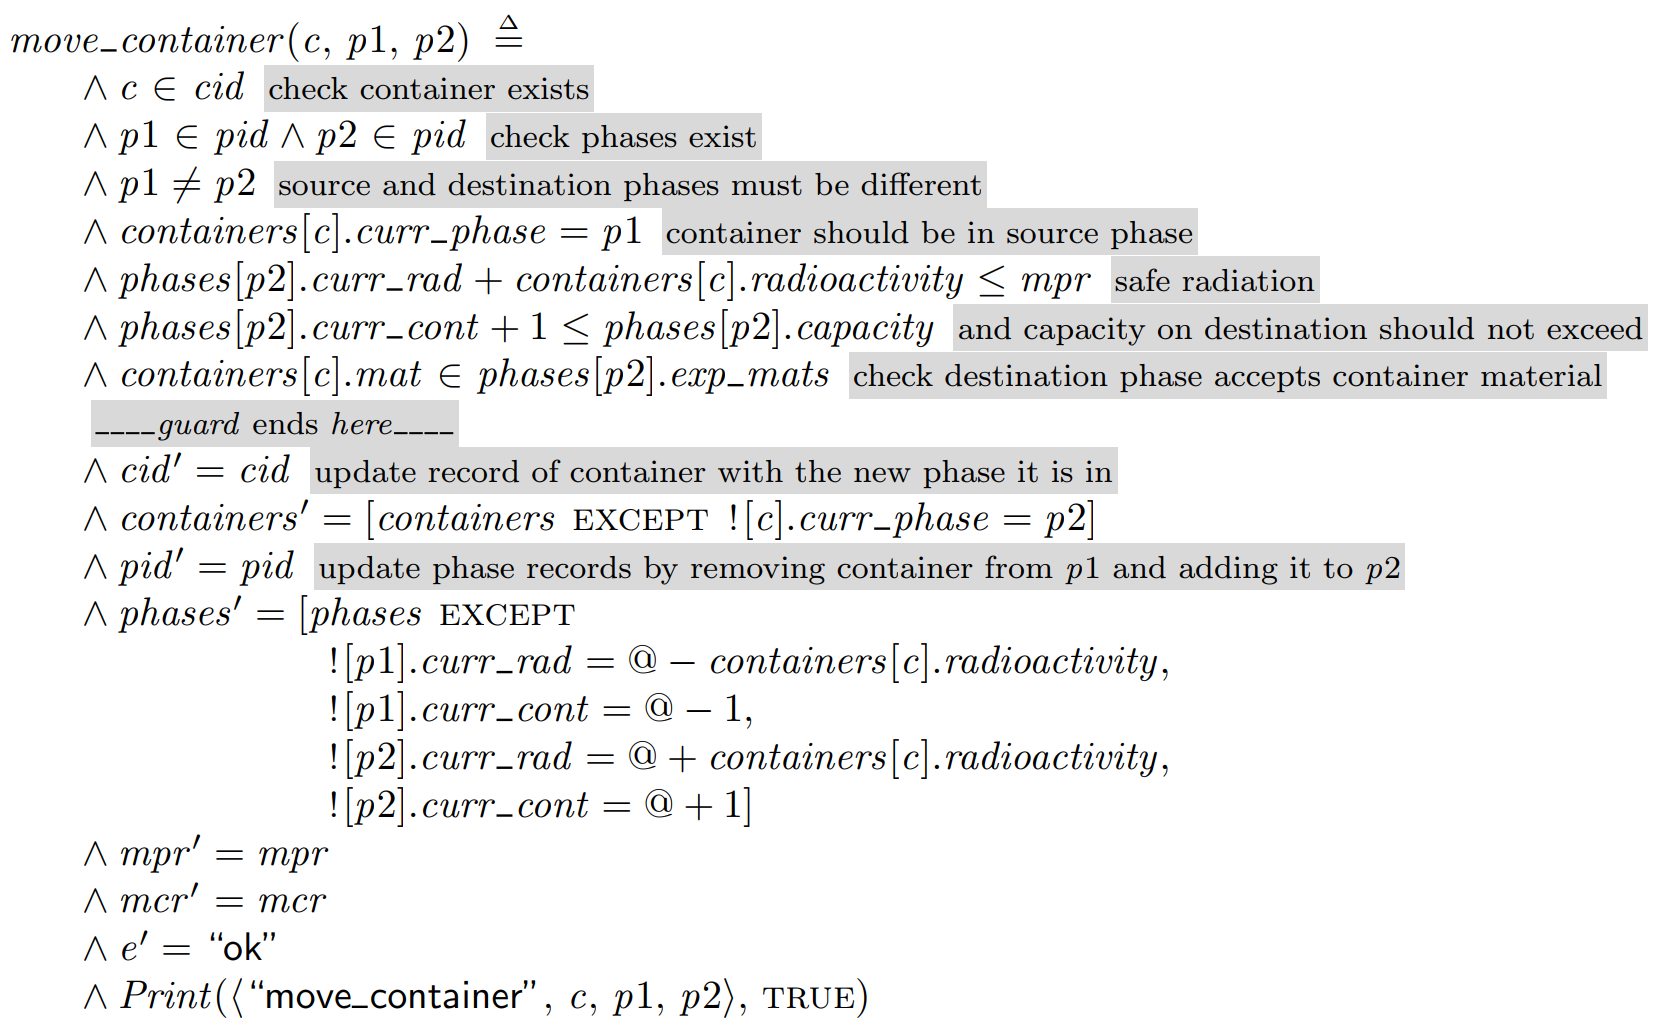
\includegraphics[width=.99\textwidth]{images/move_container.png}
\end{center}
\caption{Move Container Action in TLA}
\label{fig:move_container_action}
\end{figure}

\newpage

\subsection{TLC Model Checker}

The initial predicate and next-state relation is below:


\begin{figure}[!htb]
\begin{center}
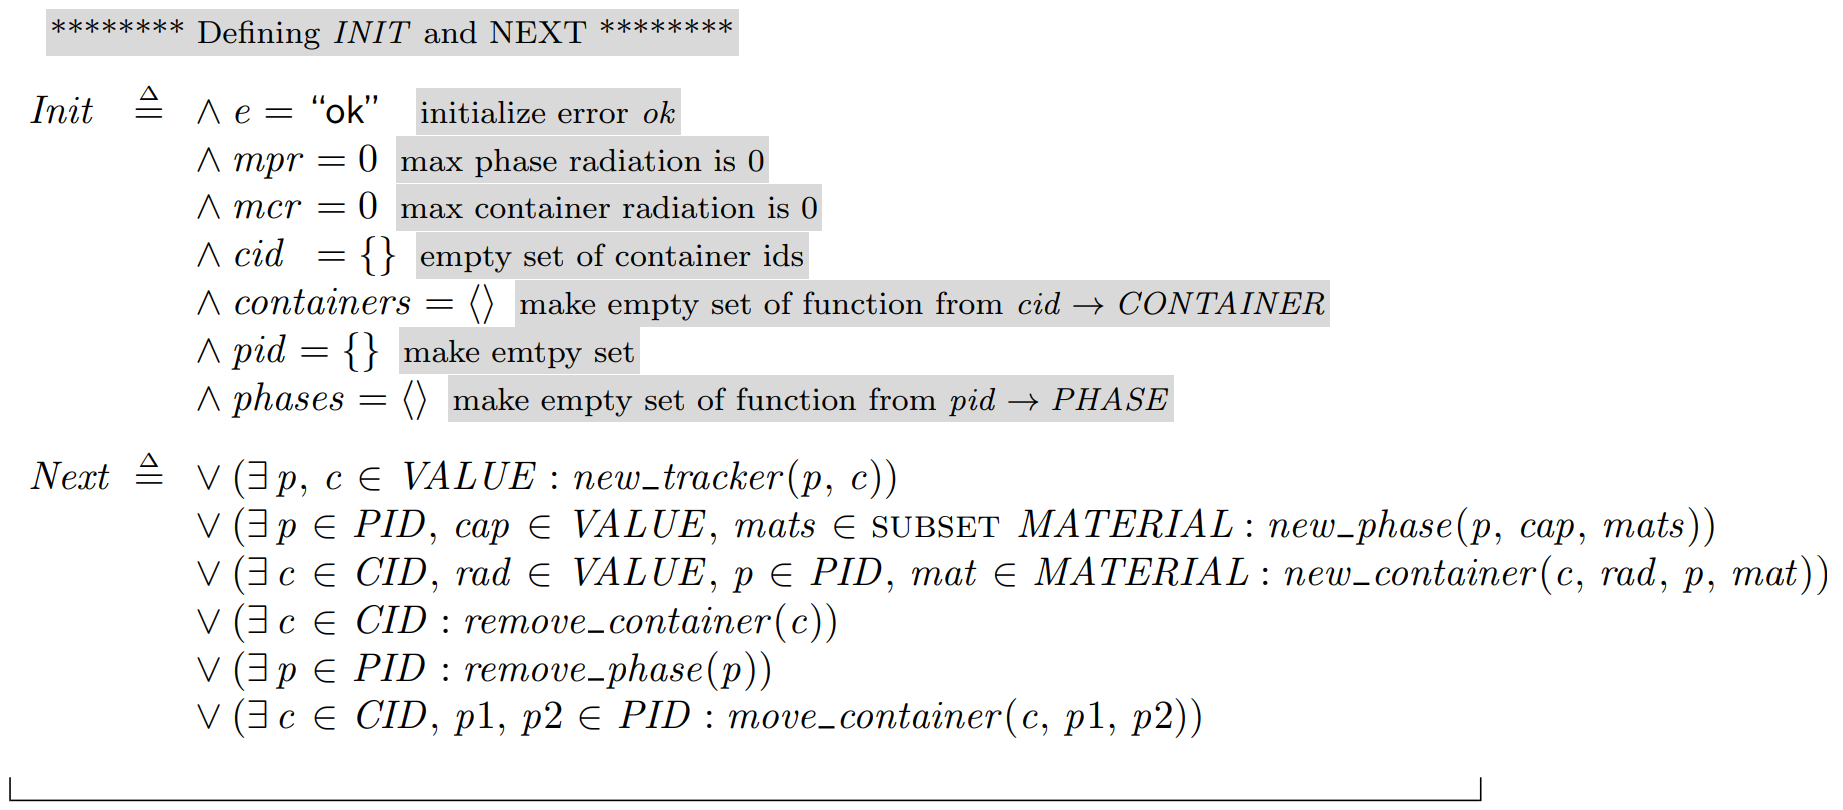
\includegraphics[width=.99\textwidth]{images/init_next.png}
\end{center}
\caption{Initial predicate and Next-State Relation}
\label{fig:init_next}
\end{figure}


\newpage
When running the model checker, it was set to check for Deadlock, and to check the invariants for the system. The following configuration was used:

\begin{figure}[!htb]
\begin{center}
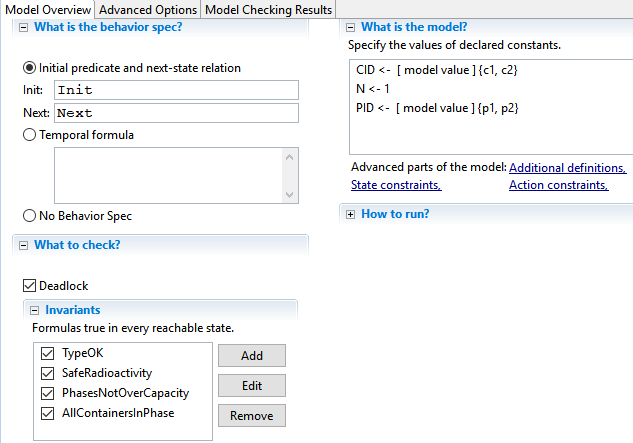
\includegraphics[width=.99\textwidth]{images/model_config.png}
\end{center}
\caption{TLA Model Checker Configuration}
\label{fig:model_config}
\end{figure}

Increasing $N$ to more than 1 or adding more values to the mode for $CID$ or $PID$ (i.e. c3, c4, ..) makes the test run for more than one hour. 

\newpage

With the configuration above, the model checker takes about 1 minute to run on a system with specs: Intel Core i7-7820HQ 2.9 GHz with 16 GB RAM. The output is seen below.
\begin{figure}[!htb]
\begin{center}
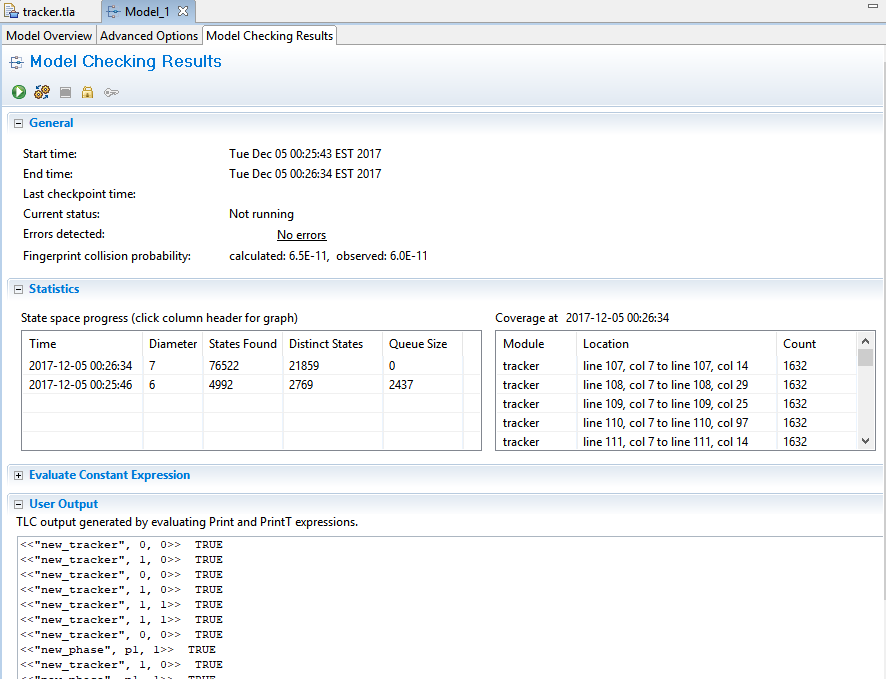
\includegraphics[width=.99\textwidth]{images/tlc_output.png}
\end{center}
\caption{TLA Model Checker Output}
\label{fig:model_config_output}
\end{figure}

\newpage
%%%%%%%%%%%%%%%%%%%%%%%%%%%%%%%%%%%%%%%%%%%%%%%%%%%%%%%%%%%%%%%%%%%%%%%%
\newpage
\section{Completeness, disjointness and well-definednes of the specification}

\begin{table}[h]
\centering
\begin{tabular}{| c | c | c | c | c | c | c | c | c | c | c | c |}
	\cline{6-12}
	\multicolumn{5}{ c| }{ }& pid & cid & phases & containers & mpr & mcr  & err \\ \hline
	\multicolumn{5}{ |c| }{ $ i= 0$}& $\{\}$ & $\{\}$ & $<>$ & $<>$ & $0$ & $0$ & "ok" \\ \cline{1-12}
	{\multirow{6}{*}{$i>0$}}  &  
	
	{\multirow{2}{*}{$new\_tracker(p, c)(i)$}} & \multicolumn{3}{ c| }{ $G1$} & \multicolumn{4}{c|}{NC} & \textbf{p} & \textbf{c} & NC\\ \cline{3-12}
	& & \multicolumn{3}{ c| }{ $\neg G1$} & \multicolumn{6}{c|}{NC} & E1\\ \cline{2-12}
	
	& {\multirow{2}{*}{$new\_phase(p, cap, mats)(i)$}} & \multicolumn{3}{ c| }{ $G2$} & C1 & NC & C2 & \multicolumn{4}{c|}{NC}\\ \cline{3-12}
	& & \multicolumn{3}{ c| }{ $\neg G2$} & \multicolumn{6}{c|}{NC} & E2\\ \cline{2-12}
	
	& {\multirow{2}{*}{$new\_container(c, rad, p, m)$}} & \multicolumn{3}{ c| }{ $G3$} & NC & C3 & C4 & C5 & \multicolumn{3}{c|}{NC}\\ \cline{3-12}
	& & \multicolumn{3}{ c| }{ $\neg G3$} & \multicolumn{6}{c|}{NC} & E3\\ \cline{2-12}
	
	& {\multirow{2}{*}{$remove\_container(c)$}} & \multicolumn{3}{ c| }{ $G4$} & NC & C6 & C7 & C8 & \multicolumn{3}{c|}{NC}\\ \cline{3-12}
	& & \multicolumn{3}{ c| }{ $\neg G4$} & \multicolumn{6}{c|}{NC} & E4\\ \cline{2-12}
	
	& {\multirow{2}{*}{$remove\_phase(p)$}} & \multicolumn{3}{ c| }{ $G5$} & C9 & NC & C10 & \multicolumn{4}{c|}{NC}\\ \cline{3-12}
	& & \multicolumn{3}{ c| }{ $\neg G5$} & \multicolumn{6}{c|}{NC} & E5\\ \cline{2-12}
	
	& {\multirow{2}{*}{$move\_container(c, p1, p2)$}} & \multicolumn{3}{ c| }{ $G6$} & \multicolumn{2}{c|}{NC} & C11 & C12 & \multicolumn{3}{c|}{NC}\\ \cline{3-12}
	& & \multicolumn{3}{ c| }{ $\neg G6$} & \multicolumn{6}{c|}{NC} & E6\\ \cline{2-12} \hline
\end{tabular}
\caption {Function Table for the actions in the TLA+ specification}
\label{tbl:ft_spec}
\end{table}

\begin{table}[h]
\centering
\begin{tabular}{| c | c | }
	\cline{1-2}
	\textbf{Guards} & \textbf{Value} \\ \hline
	G1 & $p >= 0 \land c >= 0 \land p >= c \land cid = \{\}$ \\ \hline
	G2 & $p \notin pid \land cap > 0 \land mats \subseteq MATERIAL \land cid = \{\}$ \\ \hline
	G3 & $c \notin cid \land p \notin pid \land rad >= 0 \land rad <= mcr \land $ 
	\\ & $phases[p].curr\_rad + rad <= mpr \land phases[p].curr\_cont + 1 <= $ 
	\\ & $phases[p].capacity \land m \in MATERIAL \land m \in phases[p].exp\_mats$ \\ \hline
	G4 & $c \in cid$ \\ \hline
	G5 & $p \in pid \land cid = \{\}$ \\ \hline
    G6 & $c \in cid \land p1 \in pid \land p2 \in pid \land p1 \neq p2 \land$ 
    \\ & $phases[p2].curr\_rad + containers[c].radioactivity <= mpr \land$ 
    \\ & $phases[p2].curr\_cont + 1 <= phases[p2].capacity \land$ 
    \\ & $containers[c].mat \in phases[p2].exp\_mats$ \\ \hline
\end{tabular}
\caption {Guards described in the TLA+ specification}
\label{tbl:guards}
\end{table}

\newpage

\begin{table}[h]
\centering
\begin{tabular}{| c | c | }
	\cline{1-2}
	\textbf{Conditions} & \textbf{Value} \\ \hline
	C1 & $pid \bunion \{p\}$ \\ \hline
	C2 & $phases@@p:>[capacity |-> cap, curr\_cont |-> 0, curr\_rad |-> 0,$ 
	\\ & $exp\_mats |-> mats]$ \\ \hline
	C3 & $cid \bunion \{c\}$ \\ \hline
	C4 & $[phases$ EXCEPT $![p].curr\_rad = @ + rad, ![p].curr\_rad = @ + 1]$ \\ \hline
	C5 & $containers@@c:>[radioactivity |-> rad, curr\_phase |-> p, mat |-> m$ \\ \hline
    C6 & $cid \setminus \{c\}$ \\ \hline
    C7 & $[phases$ EXCEPT $![containers[c].curr\_phase].curr\_rad = $ 
    \\ & $@ - containers[c].radioactivity, ![containers[c].curr\_phase].curr\_cont = $ 
    \\ & $@ - 1]$ \\ \hline
    C8 & $DomSub(\{c\}, containers)$ \\ \hline
    C9 & $pid \setminus \{p\}$ \\ \hline
    C10 & $DomSub(\{p\}, phases)$ \\ \hline
    C11 & $[phases$ EXCEPT $![p1].curr\_rad = @ - containers[c].radioactivity, $ 
    \\ & $![p1].curr\_cont = @ - 1, ![p2].curr\_rad = @ - containers[c].radioactivity, $ 
    \\ & $![p2].curr\_cont = @ - 1]$ \\ \hline
    C12 & $[containers$ EXCEPT $![c].curr\_phase = p2]$ \\ \hline
\end{tabular}
\caption {Transformation functions for each variable described in the TLA+ specification}
\label{tbl:conds_spec}
\end{table}

The error messages used in the TLA+ specification relates to the error messages specified by the customer during the elicitation phase refer to Table \ref{tbl:err}. Below is the table of relation between the error messages described in the TLA+ specification and the customer elicited error messages.\\

\begin{table}[h]
\centering
\begin{tabular}{| c | c | }
	\cline{1-2}
	\textbf{Error Messages} & \textbf{Value} \\ \hline
	E1 & $E1 \in \{e1, e2, e3, e4\}$ \\ \hline
	E2 & $E2 \in \{e1, e5, e6, e7, e8\}$ \\ \hline
	E3 & $E3 \in \{e5, e9, e10, e11, e12, e13, e14, e18\}$ \\ \hline
	E4 & $E4 \in \{e15\}$ \\ \hline
	E5 & $E5 \in \{e1, e9\}$ \\ \hline
    E6 & $E6 \in \{e9, e11, e12, e13, e15, e16, e17$ \\ \hline
\end{tabular}
\caption {Errors described in the TLA+ specification}
\label{tbl:error_spec}
\end{table}


%%%%%%%%%%%%%%%%%%%%%%%%%%%%%%%%%%%%%%%%%%%%%%%%%%%%%%%%%%%%%%%%%%%%%%%%
\newpage
\section{Analysis of required status and error messages}
Table below shows the value for each error message:

\bigskip

\begin{table}[h]
\centering
\begin{tabular}{|c|c|}
	\cline{2-2}
	\multicolumn{1}{ c| }{ } & \textbf{Message} \\ \hline
	e1 & current tracker is in use \\ \hline
	e2 & max phase radiation must be non-negative value \\ \hline
	e3 & max container radiation must be non-negative value \\ \hline
	e4 & max container must not be more than max phase radiation \\ \hline
	e5 & identifiers/names must start with A-Z, a-z or 0..9 \\ \hline
    e6 & phase identifier already exists \\ \hline
    e5 & identifiers/names must start with A-Z, a-z or 0..9 \\ \hline
    e7 & phase capacity must be a positive integer \\ \hline
    e8 & there must be at least one expected material for this \\ \hline
    e9 & phase identifier not in the system \\ \hline
    e10 & this container identifier already in tracker \\ \hline
    e11 & this container will exceed phase capacity \\ \hline
    e12 & this container will exceed phase safe radiation \\ \hline
    e13 & phase does not expect this container material \\ \hline
    e14 & container radiation capacity exceeded \\ \hline
    e15 & this container identifier not in tracker \\ \hline
    e16 & source and target phase identifier must be different \\ \hline
    e17 & this container identifier is not in the source phase \\ \hline
    e18 & this container radiation must not be negative \\ \hline
    ELSE & ok \\ \hline
\end{tabular}
\caption {Description table for error messages}
\label{tbl:err}
\end{table}



%%%%%%%%%%%%%%%%%%%%%%%%%%%%%%%%%%%%%%%%%%%%%%%%%%%%%%%%%%%%%%%%%%%%%%%%
\newpage
\section{Acceptance Tests}
%%%%%%%%%%%%%%%%%%%%%%%%%%%%%%%%%%%%%%%%%%%%%%%%%%

The table below describes the relationship between the use cases and concrete acceptance tests developed for the system:

\begin{table}[!ht]
\centering
\begin{tabular}{|l|l|l|}
\hline
Use Cases & Description & Acceptance Tests \\ \hline
\multirow{2}{*}{UC-1} & \multirow{2}{*}{Moving a container} & at1.txt \\ \cline{3-3} 
 &  & at3.txt \\ \hline
\multirow{2}{*}{UC-2} & \multirow{2}{*}{Permission for moving a container} & at1.txt \\ \cline{3-3} 
 &  & at3.txt \\ \hline
\multirow{3}{*}{UC-3} & \multirow{6}{*}{Creating a new tracker} & at1.txt \\ \cline{3-3} 
 &  & at2.txt \\ \cline{3-3}
 &  & at3.txt \\ \cline{3-3} 
 &  & at4.txt \\ \cline{3-3} 
 &  & at5.txt \\ \cline{3-3} 
 &  & at6.txt \\ \hline
\multirow{2}{*}{UC-4} & \multirow{2}{*}{Creating a new phase} & at4.txt \\ \cline{3-3} 
  &  & at5.txt \\ \cline{3-3}
 &  & at6.txt \\ \hline
\multirow{2}{*}{UC-5} & \multirow{3}{*}{Creating a new container} & at4.txt \\ \cline{3-3} 
 &  & at5.txt \\ \cline{3-3}
 &  & at6.txt \\ \hline
\multirow{2}{*}{UC-6} & \multirow{2}{*}{Removing a container} & at2.txt \\ \cline{3-3} 
	&  & at4.txt \\ \cline{3-3} 
 &  & at5.txt \\ \hline
\multirow{2}{*}{UC-7} & \multirow{2}{*}{Removing a phase} & at2.txt \\ \cline{3-3} 
	&  & at4.txt \\ \cline{3-3} 
 &  & at5.txt \\ \hline
\end{tabular}
\caption{Acceptance Tests for each Use Case}
\label{my-label}
\end{table}

%%%%%%%%%%%%%%%%%%%%%%%%%%%%%%%%%%%%%%%%%%%%%%%%%%%%%%%%%%%%%%%%%%%%%%%%
\newpage
\section{Traceability Matrix}
%%%%%%%%%%%%%%%%%%%%%%%%%%%%%%%%%%%%%%%%%%%%%%%%%%

The table below traces which R-descriptions are tested by which acceptance tests:

\begin{table}[h]
\centering
\begin{tabular}{| c | c | c | c | c | c | c |}
	\cline{1-7}
	\textbf{REQ} & \textbf{a1.txt} & \textbf{a2.txt} & \textbf{a3.txt} & \textbf{a4.txt} & \textbf{a5.txt} & \textbf{a6.txt} \\ \hline
	REQ1 & X & X & X & X & X & X \\ \hline
	REQ2 & & & & X & X & X \\ \hline
	REQ3 & & & & X & X & X \\ \hline
	REQ4 & & & & X & X & X \\ \hline
	REQ5 & & X & X & X & & \\ \hline
\end{tabular}
\caption {Traceability Matrix for R-descriptions}
\label{tbl:trace_matrix}
\end{table}

%%%%%%%%%%%%%%%%%%%%%%%%%%%%%%%%%%%%%%%%%%%%%%%%%%%%%%%%%%%%%%%%%%%%%%%%
\newpage
\section{Requirements Elicitation}

Our abstract UI grammar in Phase1 was similar to the abstract UI grammar provided by our customer in Phase2. However there were some major discrepancies between now and our initial elicitation of the customer needs:

\smallskip

\begin{mylist}
\item We assumed that when creating a new container, the radioactivity value of the container could be negative.
\item We assumed that when moving a container, it was not necessary to know the source phase.
\item Our initial abstract grammar used a tuple to represent Containers with all the values needed to create a container, whereas the customer's representation included only the material and radiation value.
\item Our initial abstract grammar used a tuple to represent Phases, whereas the customer's representation did not have any tuple for Phases.
\end{mylist}
%%%%%%%%%%%%%%%%%%%%%%%%%%%%%%%%%%%%%%%%%%%%%%%%%%

\newpage
\section{Appendices}
\appendix

\section{TLA}	\label{tla-spec}
The following pages include the TLA+ specification for the System Under Description:
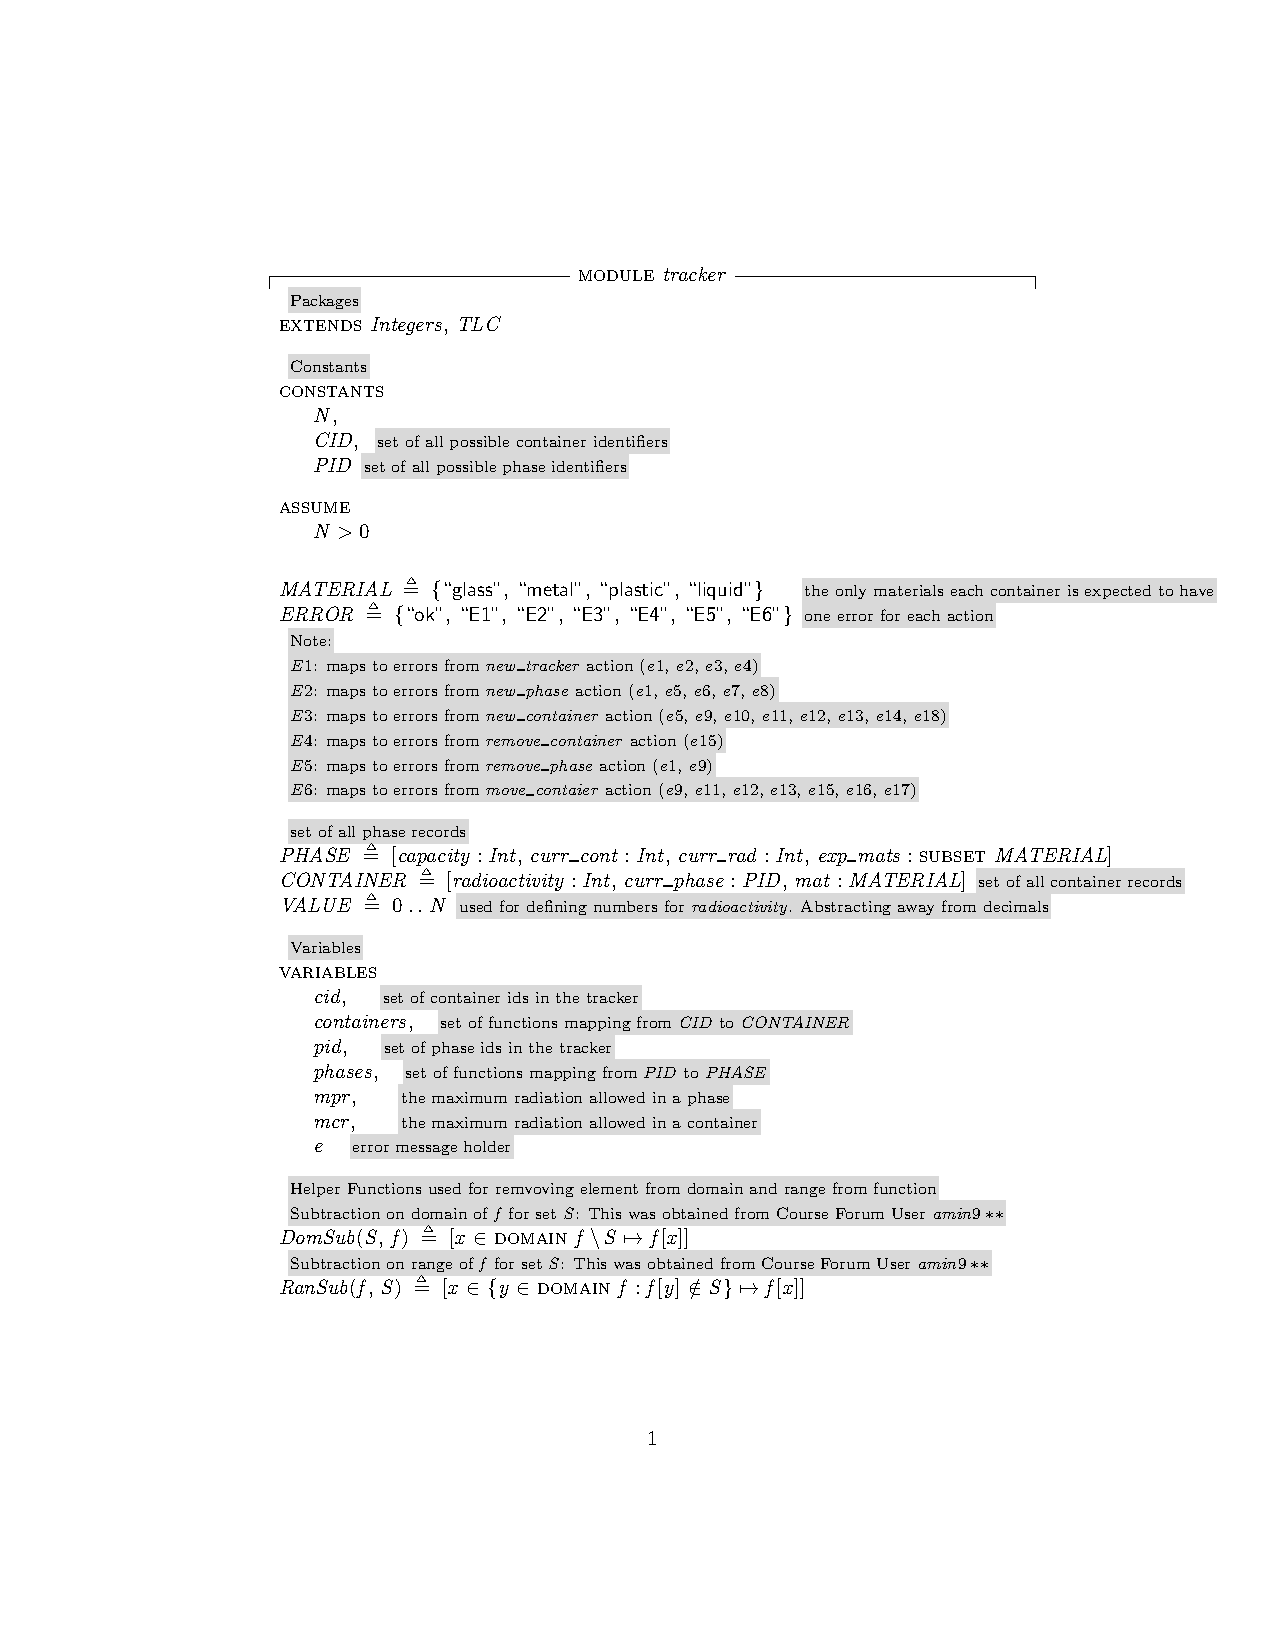
\includepdf[pages={1-}]{../../tla/tracker.pdf}

\section{Additional R-Descriptions}	\label{add-rdesc}

Below are additional R-Descriptions for the System Under Description:

\rdescription
{An error message shall be signalled if a container is registered with a radiation value greater than the plant's maximum radiation limit.\\}
{}
\label{R4}

\smallskip
\noindent \textbf{Rationale}: It is dangerous to allow having a container in the system with a radiation value that exceed the plant's maximum radiation limit. Whenever a new container with a radiation value greater than the plant's maximum radiation limit is attempted to be added to the plant, an error shall be signalled to the operator.

\rdescription
{A phase may also be removed if there are no containers in the plant.\\}
{}
\label{R5}

\smallskip
\noindent \textbf{Rationale}: Keeping a phase in a plant may not be necessary when there are no containers in the plant. Hence, the phase can be removed by the operator if there are no more containers left in the plant.

\newpage
\section{Additional Textual Use Cases}	\label{add-uctd}

\begin{table}[h]
\begin{center}
\begin{tabular}{|l|l|}
\hline
\textbf{Use Case ID:} UC-2 \\ \hline
\textbf{Use Case Name:} Permission for Container Movement \\ \hline
\textbf {Primary Actor:} Tracking Manager \\ \hline
\textbf{Description:} The Tracking Manager is requested to verify if a containers \\movement between two phases is safe. The Tracking Manager verifies the \\destination phases accepted materials consist of the material from the container \\and enters it. The system processes it and signals success for the \\movement of the container. \\ \hline
\textbf{Scenario:} Sunny Day \\ \hline
\textbf{Trigger:} Normal Flow 1.0.6\\ \hline
\textbf{Priority:} High \\ \hline
\textbf{Precondition:}
\\ PRE-1. Number of containers in destination phase, \emph{p2}, is less than the \\maximum containers allowed in \emph{p2}.\\ \hline
\textbf{Postcondition:}
\\ POST-1. Movement has been verified. \\ \hline
\textbf{Normal Flow:}
\\ \textbf{2.0 Permission for container, \emph{c}, to move from}
\\ \textbf{phase \emph{p1} to a phase \emph{p2}}
\\ 1. Tracking Manager is notified upon a verification request comes in \\from the system.
\\ 2. Tracking Manager verifies the destination phases accepted materials \\consist of the material in the container.
\\ 3. The Tracking Manager inputs verified.
\\ 4. System processes the input and signals success for the movement of \\the container. \\ \hline
\end{tabular}
\end{center}
\caption {UC-2 Textual Description}
\label{tbl:uc2td}
\end{table}

\begin{table}[h]
\begin{center}
\begin{tabular}{|l|l|}
\hline
\textbf{Use Case ID:} UC-3 \\ \hline
\textbf{Use Case Name:} Create a Tracker \\ \hline
\textbf {Primary Actor:} Operator \\ \hline
\textbf{Description:} The Operator specifies the option to create a tracker. The system \\prompts the operator to input the maximum phase radiation level in each phase \\in the tracker and the maximum container radiation level in each container in a \\phase in the tracker. The Operator inputs the desired values and clicks enter. \\The system processes the input and succeeds on creating the tracker. \\ \hline
\textbf{Scenario:} Sunny Day \\ \hline
\textbf{Trigger:} Operator indicates to create a tracker.\\ \hline
\textbf{Priority:} High \\ \hline
\textbf{Precondition:}
\\ PRE-1. \emph{mpr} must be greater than or equal to 0.
\\ PRE-2. \emph{mcr} must be greater than or equal to 0.
\\ PRE-3. \emph{mpr} must be greater than or equal to \emph{mcr}.
\\ PRE-4. There should not be any active containers or phases in the tracker. \\ \hline
\textbf{Postcondition:}
\\ POST-1. Tracker, \emph{t}, is created. \\ \hline
\textbf{Normal Flow:} 
\\ \textbf{3.0 Create a tracker, \emph{t} with max phase radiation,\emph{mpr} and}
\\ \textbf{max container radiation,\emph{mcr}}
\\ 1. Operator selects the option to create a tracker.
\\ 2. System prompts the Operator to enter the maximum phase radiation level \\allowed in each phase and the maximum container radiation allowed in a \\container.
\\ 3. Operator enters the max phase radiation and max container radiation \\and clicks enter.
\\ 4. System processes the input and responses OK.\\ \hline
\textbf{Exception Flow: 3.0.E1 Max Phase Radiation is negative}
\\ 1. System displays error \textbf{e2: max phase radiation must be} \\ \textbf{non-negative value}.
\\ 2. System asks the Operator if they want to input a correct max phase radiation \\value (3a) or to exit (4a).
\\ 3a. Operator requests to enter a new max phase radiation value.
\\ 3b. System starts normal flow over.
\\ 4a. Operator asks to exit.
\\ 4b. System terminates the use case.\\ \hline
\end{tabular}
\end{center}
\caption {UC-3 Textual Description}
\label{tbl:uc3td}
\end{table}

\begin{table}[h]
\begin{center}
\begin{tabular}{|l|l|}
\hline
\textbf{Use Case ID:} UC-4 \\ \hline
\textbf{Use Case Name:} Create a Phase \\ \hline
\textbf {Primary Actor:} Operator \\ \hline
\textbf{Description:} The Operator specifies the option to create a new phase. \\The system prompts the operator to input the phase ID, phase name, container \\capacity and a list of expected materials in the phase. The Operator inputs the\\ desired values and clicks enter. The system processes the input and succeeds on \\creating a new phase. \\ \hline
\textbf{Scenario:} Sunny Day \\ \hline
\textbf{Trigger:} Operator indicates to create a phase.\\ \hline
\textbf{Priority:} High \\ \hline
\textbf{Precondition:}
\\ PRE-1. Phase with \emph{pid} does not exist in the tracker.
\\ PRE-2. Name of the phase must start with A-Z, a-z or 0..9.
\\ PRE-3. Identifier of the phase must start with A-Z, a-z or 0..9.
\\ PRE-4. Phase capacity, \emph{pcap}, must be greater than 0.
\\ PRE-5. The expected materials list must have at least one material. \\ \hline
\textbf{Postcondition:}
\\ POST-1. Phase, \emph{p}, with \emph{pid} is created. \\ \hline
\textbf{Normal Flow:} 
\\ \textbf{3.0 Create a phase, \emph{p}, with \emph{pid}, \emph{pname}, \emph{pcap} and \emph{pmat}}
\\ 1. Operator selects the option to create a phase.
\\ 2. System prompts the Operator to the phase ID, phase name, container \\capacity and a list of expected materials in the phase.
\\ 3. Operator enters the desired values \\and clicks enter.
\\ 4. System processes the input and responses OK. \\ \hline
\textbf{Exception Flow: 3.0.E1 Expected materials list is empty}
\\ 1. System displays error \textbf{e8: there must be at least one expected} \\ \textbf{material for this phase}.
\\ 2. System asks the Operator if they want to input a new set of \\expected materials (3a) or to exit (4a).
\\ 3a. Operator requests to enter a new set of expected materials.
\\ 3b. System starts normal flow over.
\\ 4a. Operator asks to exit.
\\ 4b. System terminates the use case.\\ \hline
\end{tabular}
\end{center}
\caption {UC-4 Textual Description}
\label{tbl:uc4td}
\end{table}

\begin{table}[h]
\begin{center}
\begin{tabular}{|l|l|}
\hline
\textbf{Use Case ID:} UC-5 \\ \hline
\textbf{Use Case Name:} Create a Container \\ \hline
\textbf {Primary Actor:} Operator \\ \hline
\textbf{Description:} The Operator specifies the option to create a new container. \\The system prompts the operator to input the container ID, a tuple containing \\the material in the container and the radioactivity value in the container \\and the phase ID to be added to. The Operator inputs the desired values \\and clicks enter. The system processes the input and succeeds on creating \\a new container. \\ \hline
\textbf{Scenario:} Sunny Day \\ \hline
\textbf{Trigger:} Operator indicates to create a container.\\ \hline
\textbf{Priority:} High \\ \hline
\textbf{Precondition:}
\\ PRE-1. Container with \emph{cid} does not exist in the tracker.
\\ PRE-2. Phase with \emph{pid} exists in the tracker.
\\ PRE-3. Identifier of the container must start with A-Z, a-z or 0..9.
\\ PRE-4. The containers radiation must be greater than 0.
\\ PRE-5. The container must have a material type. \\ \hline
\textbf{Postcondition:}
\\ POST-1. Container, \emph{c}, with \emph{cid} is created and added to phase with \emph{pid}. \\ \hline
\textbf{Normal Flow:} 
\\ \textbf{5.0 Create a container, \emph{c}, with \emph{cid}, \emph{container} and \emph{pid}}
\\ 1. Operator selects the option to create a container.
\\ 2. System prompts the Operator to the container ID, containers radioactivity \\value and material type and phase ID it needs to be added.
\\ 3. Operator enters the desired values \\and clicks enter.
\\ 4. System processes the input and responses OK.\\ \hline
\textbf{Exception Flow: 5.0.E1}
\\ \textbf{Phase to be added to does not expect this container material}
\\ 1. System displays error \textbf{e13: phase does not expect} \\ \textbf{this container material}.
\\ 2. System asks the Operator if they want to a add another \\container with the correct expected material (3a) or to exit (4a).
\\ 3a. Operator requests to create a new container with the correct expected material.
\\ 3b. System starts normal flow over.
\\ 4a. Operator asks to exit.
\\ 4b. System terminates the use case.\\ \hline
\end{tabular}
\end{center}
\caption {UC-5 Textual Description}
\label{tbl:uc5td}
\end{table}

\begin{table}[h]
\begin{center}
\begin{tabular}{|l|l|}
\hline
\textbf{Use Case ID:} UC-6 \\ \hline
\textbf{Use Case Name:} Remove a Container \\ \hline
\textbf {Primary Actor:} Operator \\ \hline
\textbf{Description:} The Operator specifies the option to remove a container. \\The system prompts the operator to input the container ID. The \\Operator inputs the ID and clicks enter. The system processes the \\input and succeeds on removing the container. \\ \hline
\textbf{Scenario:} Sunny Day \\ \hline
\textbf{Trigger:} Operator indicates to remove a container.\\ \hline
\textbf{Priority:} High \\ \hline
\textbf{Precondition:}
\\ PRE-1. Container with \emph{cid} exist in the tracker.\\ \hline
\textbf{Postcondition:}
\\ POST-1. Container with \emph{cid} has been removed from the tracker. \\ \hline
\textbf{Normal Flow: 6.0 Remove a container with \emph{cid}}
\\ 1. Operator selects the option to remove a container.
\\ 2. System prompts the Operator to the enter container ID.
\\ 3. Operator enters the value \\and clicks enter.
\\ 4. System processes the input and responses OK.\\ \hline
\textbf{Exception Flow: 6.0.E1 Container to be removed is not in the tracker}
\\ 1. System displays error \textbf{e15: this container identifier} \\ \textbf{not in tracker}.
\\ 2. System asks the Operator if they want to a remove another \\container (3a) or to exit (4a).
\\ 3a. Operator requests to remove another container.
\\ 3b. System starts normal flow over.
\\ 4a. Operator asks to exit.
\\ 4b. System terminates the use case.\\ \hline
\end{tabular}
\end{center}
\caption {UC-6 Textual Description}
\label{tbl:uc6td}
\end{table}

\begin{table}[h]
\begin{center}
\begin{tabular}{|l|l|}
\hline
\textbf{Use Case ID:} UC-7 \\ \hline
\textbf{Use Case Name:} Remove a Phase \\ \hline
\textbf {Primary Actor:} Operator \\ \hline
\textbf{Description:} The Operator specifies the option to remove a container. \\The system prompts the operator to input the phase ID. The \\Operator inputs the ID and clicks enter. The system processes the \\input and succeeds on removing the phase. \\ \hline
\textbf{Scenario:} Sunny Day \\ \hline
\textbf{Trigger:} Operator indicates to remove a phase.\\ \hline
\textbf{Priority:} High \\ \hline
\textbf{Precondition:}
\\ PRE-1. Phase with \emph{pid} exist in the tracker.\\ \hline
\textbf{Postcondition:}
\\ POST-1. Phase with \emph{pid} has been removed from the tracker. \\ \hline
\textbf{Normal Flow: 7.0 Remove a phase with \emph{pid}}
\\ 1. Operator selects the option to remove a phase.
\\ 2. System prompts the Operator to the enter phase ID.
\\ 3. Operator enters the value \\and clicks enter.
\\ 4. System processes the input and responses OK.\\ \hline
\textbf{Exception Flow: 7.0.E1 Phase ID is not in the tracker}
\\ 1. System displays error \textbf{e9: phase identifier not in the system}.
\\ 2. System asks the Operator if they want to a remove another phase (3a) \\or to exit (4a).
\\ 3a. Operator requests to remove another phase.
\\ 3b. System starts normal flow over.
\\ 4a. Operator asks to exit.
\\ 4b. System terminates the use case.\\ \hline
\end{tabular}
\end{center}
\caption {UC-7 Textual Description}
\label{tbl:uc7td}
\end{table}

